\section{Développement}

\subsection{Les métadonnées}

\begin{frame}
	\frametitle{\insertsubsectionhead}
	\begin{block}{Des métadonnées en communs}
		\begin{itemize}
		\item Le \textit{MAGIC}
		\item Version
		\item Algorithme de chiffrement et de hashage
		\item Sel
		\item Nombre d'itérations pour PKCS5v2
		\item Clé maître chiffrée
		\end{itemize}
	\end{block}
\end{frame}

\begin{frame}
	\frametitle{\insertsubsectionhead - \textbf{FreeBSD}}
	\begin{figure}
		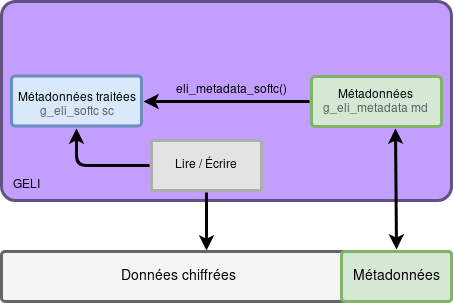
\includegraphics[width=.8\textwidth]{developpement/utilisation_metadonnee}
		\caption{Utilisation des métadonnées dans FreeBSD}
	\end{figure}
\end{frame}

\begin{frame}
	\frametitle{\insertsubsectionhead - Utilisation dans le code}
	\begin{figure}
		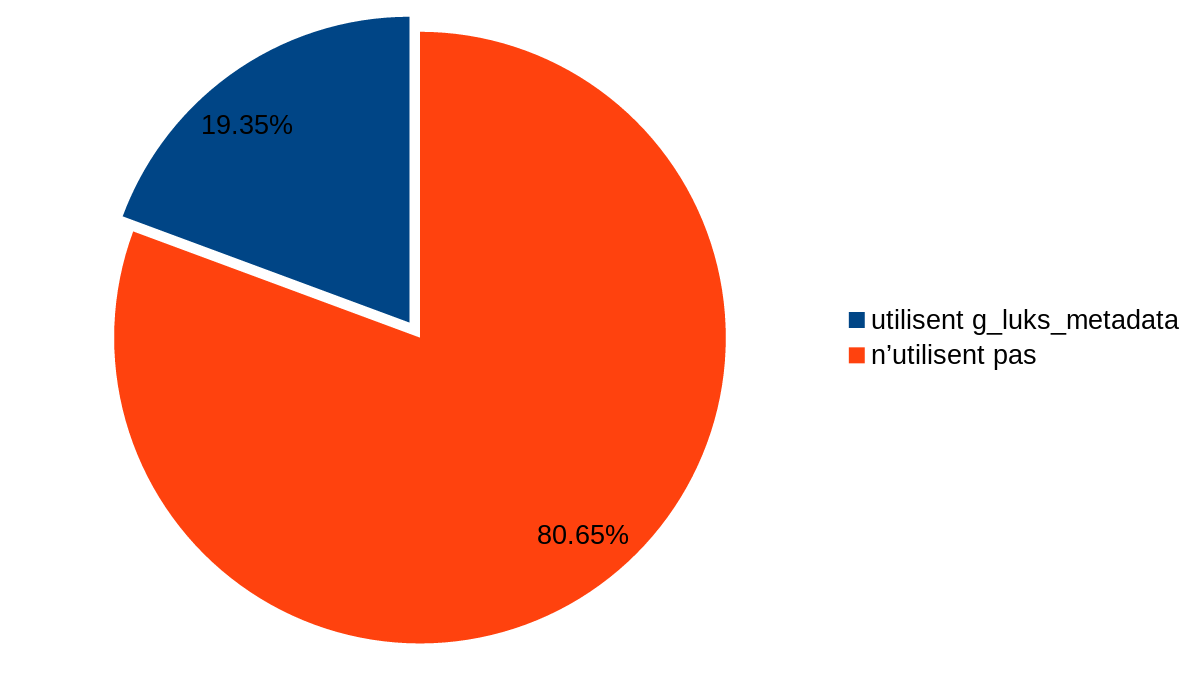
\includegraphics[width=.8\textwidth]{developpement/fonctions_g_luks_metadata}
		\caption{Utilisation de la structure g\_luks\_metadata}
	\end{figure}
\end{frame}
\begin{frame}
	\frametitle{\insertsubsectionhead - Utilisation dans le code}
	\begin{figure}
		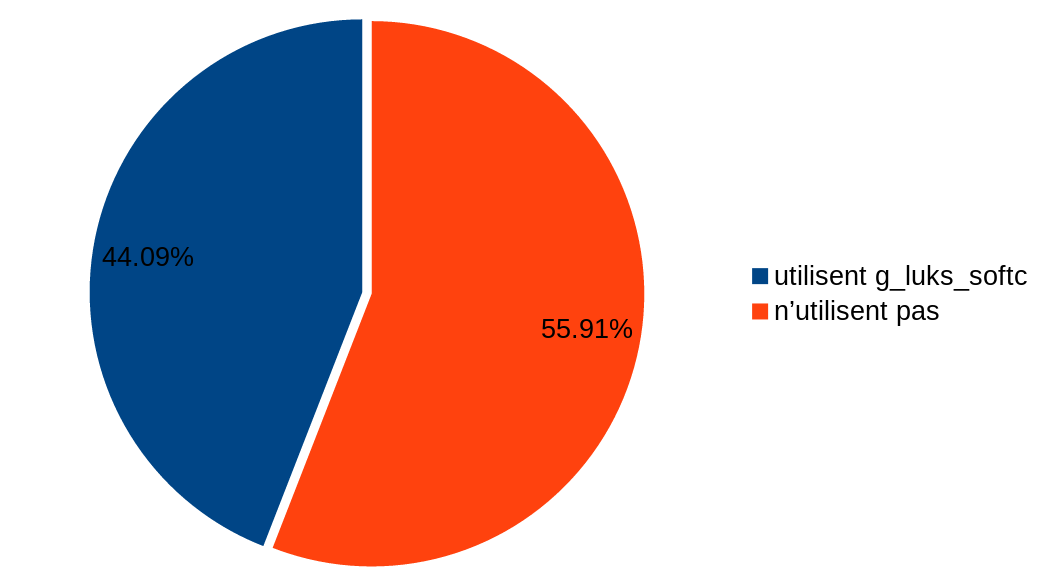
\includegraphics[width=.8\textwidth]{developpement/fonctions_g_luks_softc}
		\caption{Utilisation de la structure g\_luks\_softc}
	\end{figure}
\end{frame}

\begin{frame}
	\frametitle{\insertsubsectionhead - Transformation des métadonnées}
	\begin{figure}
		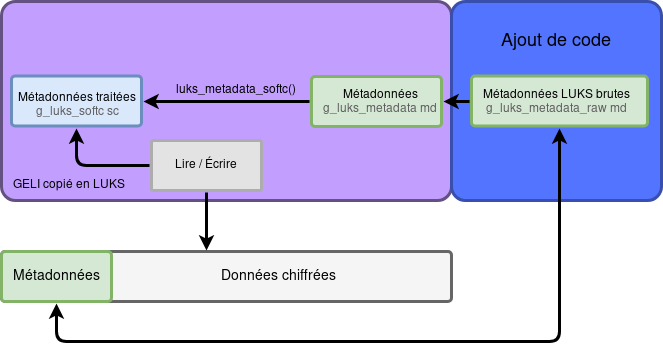
\includegraphics[width=\textwidth]{developpement/utilisation_metadonnee_luks}
		\caption{Introduction d'un structure intermédiaire}
	\end{figure}
\end{frame}

\subsection{Déchiffrement de la clé}

\begin{frame}
	\frametitle{\insertsubsectionhead}
	\begin{figure}
		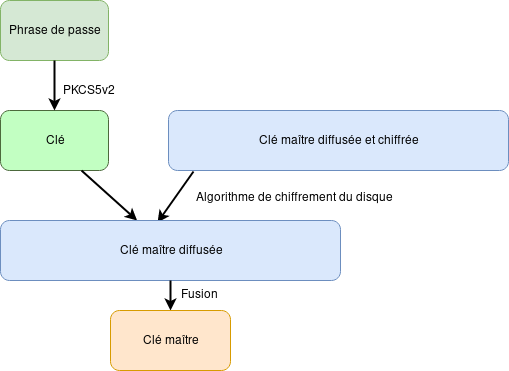
\includegraphics[width=.7\textwidth]{developpement/dechiffrement_cle}
		\caption{Déchiffrement de la clé sous LUKS}
	\end{figure}
\end{frame}

\subsection{Utilisation de drapeaux \textit{GELI}}

\begin{frame}
  \frametitle{\insertsubsectionhead}
  \begin{block}{Activer/désactiver options de chiffrement de disques}
    \begin{itemize}
    \item \texttt{G\_ELI\_FLAG\_AUTH} \\
      \textrightarrow{} activer l'auhentification
    \item \texttt{G\_ELI\_FLAG\_SINGLE\_KEY} \\
      \textrightarrow{} utiliser la même clé maître pour tous les secteurs
    \end{itemize}
  \end{block}
\end{frame}

\subsection{Création du disque déchiffré}

\begin{frame}
	\frametitle{\insertsubsectionhead}
	\begin{block}{Quelques changements par rapport à \textit{GELI}}
		\begin{itemize}
			\item Taille du disque
				\pause
			\item Décalage
				\pause
			\item Lecture de métadonnées au début du disque
		\end{itemize}
	\end{block}
\end{frame}

\subsection{Passage de l'espace utilisateur au noyau}

\begin{frame}
	\frametitle{\insertsubsectionhead}
	\begin{block}{API GEOM}
		\begin{itemize}
			\item Structure \texttt{g\_ctl\_req}
			\item Instruction \texttt{g\_ctl\_issue}
			\item Structure \texttt{g\_command}
		\end{itemize}
	\end{block}
\end{frame}

\begin{frame}
	\frametitle{\insertsubsectionhead}
	\begin{block}{Code noyau ou espace utilisateur ?}
		\begin{itemize}
			\item API noyau Opencrypto - Openssl
			\item Malloc
			\item HMAC et PKCS5v2
			\item Dérivation de la phrase de passe
		\end{itemize}
	\end{block}
\end{frame}

\begin{frame}
	\frametitle{\insertsubsectionhead - Implémentation}
	\begin{figure}
		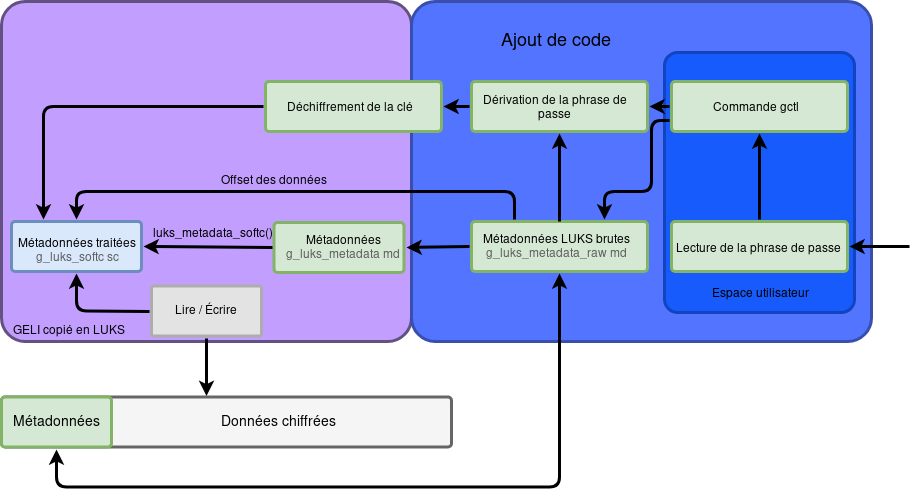
\includegraphics[width=\textwidth]{developpement/utilisation_metadonnee_luks_2}
		\caption{Fonctionnement de GEOM\_LUKS}
	\end{figure}
\end{frame}
